\section{Phase and reaction equilibrium}
\label{sec:equilibrium}
\subsection{Objective and constraints}
% P:equilibrium-01
At fixed temperature and pressure, fluid equilibrium minimizes the Gibbs energy of the declared phases,
\begin{equation}
\frac{G}{RT}=\sum_p\left[\frac{A_p}{RT}+\frac{PV_p}{RT}+\sum_i n_{p,i}\frac{g^{\circ}_{i,\rho}}{RT}\right],
\label{eq:gibbs}
\end{equation}
written in amount and volume coordinates so that no inner density solve is needed~\citep{Pereira2012}.
The minimization is subject to the conserved-moiety balances and to the electroneutrality of each phase that contains ions~\citep{Ascani2022,Tsanas2019,Tsanas2022},
\begin{equation}
\sum_pN_p\,\mathbf{B}\,\mathbf{x}_p=\mathbf{B}\,\mathbf{n}_{\mathrm{feed}},\qquad
\mathbf{z}\cdot\mathbf{x}_p=0,
\label{eq:balances}
\end{equation}
where the rows of $\mathbf{B}$ span the conserved moieties, the reactions span its null space, and every reaction conserves charge.
One electroneutrality row is omitted for a phase of nonzero amount, because the balances and the neutral feed imply it.
Without reactions $\mathbf{B}$ is the identity and Eq.~\eqref{eq:balances} reduces to species balances.
Balance rows replace reaction extents as coordinates, and the extents can be reconstructed from a solution.

% P:equilibrium-02
The first-order conditions of this minimum are, for every species $i$ on the support of phase $p$,
\begin{equation}
\mu_{p,i}-\boldsymbol{\lambda}\cdot\mathbf{B}_i-z_i\varphi_p=0,\qquad P_p(T,V_p,\mathbf{n}_p)=P,
\label{eq:stationarity}
\end{equation}
with balance multipliers $\boldsymbol\lambda$ and a charge multiplier $\varphi_p$ per phase, both in \si{\joule\per\mol}~\citep{Ascani2022,Pereira2012}.
Equal chemical potentials across phases and zero affinity, $\sum_i\nu_i\mu_{p,i}=0$, of every reaction $\boldsymbol\nu$ in the null space of $\mathbf{B}$ follow from Eq.~\eqref{eq:stationarity}; for ions, only electrochemical potentials are equal, and $\varphi_p$ corresponds to the phase potential $-F\psi_p$ up to a common gauge.
Each phase also satisfies its normalization $\sum_ix_{p,i}=1$.

% P:equilibrium-03
A specification is data on these rows, not a separate solver.
A phase amount may be free or pinned, for example at zero amount for an incipient phase, and temperature or pressure may be free.
With $k$ pinned amounts, $f$ free intensive variables and $e$ independent caloric rows, a square system requires $f=k+e$.
Temperature--pressure flashes, bubble and dew points, vapor fractions, pure-fluid saturation, critical-equation candidates, phase envelopes and pressure--enthalpy and pressure--entropy flashes are specifications of this one formulation (Table~\ref{tab:specifications}).
Reactions and ions are admitted in flashes and phase boundaries; critical-equation, envelope and pressure--enthalpy or pressure--entropy specifications are neutral, and no internal-energy--volume specification is provided.
Pinned amounts and caloric rows turn the minimization into a feasibility problem on the same intensive rows.
Pure stoichiometric solids enter the same objective through their standard Gibbs energy, with an amount complementarity at fixed temperature and pressure; no solid result is reported in this work.

\begin{table}[pos=htbp]
\centering\small
\caption{Specifications of the common equilibrium equations. $N_p$ denotes a phase amount; a zero-pinned phase is incipient. Reactions and ions are admitted in the ordinary flash and boundary declarations. Caloric, critical and envelope cases shown here are neutral.}
\label{tab:specifications}
\begin{tabularx}{\linewidth}{@{}p{0.25\linewidth}p{0.27\linewidth}X@{}}
\toprule
Specification & Fixed quantities & Free quantities and additional equations \\
\midrule
Temperature--pressure flash & $T,P$, feed, phase supports & Phase compositions, volumes and amounts \\
Bubble or dew pressure & $T$, feed, one $N_p=0$ & $P$ and incipient composition \\
Bubble or dew temperature & $P$, feed, one $N_p=0$ & $T$ and incipient composition \\
Specified phase fraction & $T$ or $P$, feed, one pinned $N_p$ & One intensive variable and all phase compositions \\
Pure saturation & $T$, pure feed, one $N_p=0$ & Common $P$ and distinct phase densities \\
Pressure--enthalpy or pressure--entropy flash & $P$, feed, extensive $H$ or $S$ & $T$, phase split and one caloric balance \\
Critical-equation candidate & Neutral composition and mode normalization & $T,P$, density and critical mode; zero quadratic and cubic forms \\
Phase envelope & Neutral feed, one $N_p=0$, one local path condition & $T,P$ and both compositions along continuation \\
\bottomrule
\end{tabularx}
\end{table}

\subsection{Coordinates, initialization and iteration}
\label{sec:driver}
% P:equilibrium-04a
Compilation reduces the conservation rows to independent balances, resolves the species allowed in each phase and checks the equation count.
For fluid phases, logarithmic compositions and packing fractions preserve their positivity and represent composition and volume.
Free phase amounts remain physical amount coordinates, scaled within the optimizer; free intensive variables and balance/charge multipliers complete the unknown vector.
Amounts and balance residuals scale with the feed basis, while chemical rows use $RT$ and pressure rows use the corresponding thermal density scale.
The logarithmic compositions have a lower bound that depends on each species' available inventory; it keeps the optimizer's coordinates finite and is not a minimum physical concentration.
The balance matrix supplies attainable amounts through linear programs, so a tiny available inventory need not be displaced by a uniform composition bound.

% P:equilibrium-04b
Initialization uses the declaration before solving its coupled equations.
For an eligible neutral two-phase temperature--pressure flash, feed-state fugacity estimates give $K_i=\phi_i^L/\phi_i^V$, and a bracketed Rachford--Rice root supplies
\begin{equation}
\sum_i\frac{z_i(K_i-1)}{1-\beta+\beta K_i}=0,\qquad
x_i=\frac{z_i}{1-\beta+\beta K_i},\quad y_i=K_ix_i.
\label{eq:rr-start}
\end{equation}
These estimates initialize amounts and compositions, after which the actual density roots are resolved.
Reacting starts first estimate liquid speciation by an ideal-solution element-potential iteration with frozen nonideal terms~\citep{gordonComputerProgramCalculation1994}.
A cold reacting incipient boundary can solve its finite phases at the pressure seed before forming the boundary start.
The seed is an estimate of the same equations, not an equilibrium conclusion or a measured phase composition.
A supplied start overrides the generated quantities it declares.

% P:equilibrium-04c
One driver solves the rows of Eqs.~\eqref{eq:balances} and~\eqref{eq:stationarity}, with first and second derivatives of the same Helmholtz energy.
For eligible ordinary calls it first applies an exact Newton iteration, factorized by full-pivot LU, with at most two step halvings.
This attempt covers neutral, nonreacting liquid/vapor boundaries with one zero-pinned amount and one free intensive variable, and full-positive-support two-phase temperature--pressure flashes.
Declared-start calls, continuation correctors, stability trials and caloric seed solves use Ipopt alone.
An admitted Newton result must satisfy the final residual, topology, density-branch and local checks.
Otherwise Ipopt~\citep{Wachter2006} solves the same rows from the original start using the exact Hessian of the Lagrangian.
When all phase amounts are free, Ipopt minimizes Eq.~\eqref{eq:gibbs} subject to Eq.~\eqref{eq:balances}, so Eq.~\eqref{eq:stationarity} are its first-order conditions; when an amount is pinned or a caloric or critical row is added, the objective is constant and every row is an equality constraint of a square feasibility problem.
Algorithm~\ref{alg:equilibrium} summarizes the sequence.

\begin{algorithm}[tbp]
\caption{A declared phase and reaction equilibrium}
\label{alg:equilibrium}
\begin{algorithmic}[1]
\Require Feed, phases and supports, reactions/references, pinned amounts, intensive and caloric data
\State Compile independent balances, references, coordinates, bounds and residual scales.
\State Construct a supplied or physical start; use speciation and phase estimates in their admitted domains.
\If{the ordinary neutral declaration admits the Newton attempt}
\State Solve the exact row Jacobian; damp within bounds and test the full final admission.
\State Return only if all requested criteria and branch checks are met.
\EndIf
\State Run Ipopt from the original start with exact constraint and Lagrangian derivatives.
\State Polish the returned positive point with contracting exact-Jacobian corrections.
\State Recompute balance, charge, normalization, pressure and stationarity defects.
\State Check distinct phases, density identity and local reduced curvature.
\If{a neutral, nonreacting liquid/vapor solve without a supplied start has failed}
\State Seek a lower-temperature source and correct back within the bounded shared work.
\State Reapply the target declaration's residual and branch checks.
\EndIf
\State Return the achieved quantities and unmet criteria, or the complete cause of no finite state.
\end{algorithmic}
\end{algorithm}

% P:equilibrium-04d
Ipopt stops on its own scaled optimality measure, which can leave the recomputed defining rows slightly above the requested tolerance; the polish removes that remainder.
The final polish accepts exact-Jacobian corrections only when raw defining-equation defects decrease and the point remains positive.
Trace balances are judged relative to their available inventory as well as on the feed scale.
Polish can extend beyond the ordinary step count while raw defects exceed the requested tolerance and work remains.
Table~\ref{tab:defaults} distinguishes caller-configurable accuracy criteria from budgets and policy constants.
A finite candidate that misses the requested accuracy remains explicitly identified.


\begin{table}[pos=htbp]
\centering\small
\caption{Default numerical criteria and budgets. The association, reduced-pressure and equilibrium-row residual tolerances are caller-configurable and dimensionless after the stated normalization. The other rows give work budgets and fixed policy values, including the polish and implicit-action criteria. Budgets bound work; initialization and separation constants do not certify accuracy.}
\label{tab:defaults}
\begin{tabularx}{\linewidth}{@{}p{0.34\linewidth}p{0.16\linewidth}X@{}}
\toprule
Quantity & Default & Meaning \\
\midrule
Association residual & $2\times10^{-13}$ & Infinity norm of the mass-action equations \\
Association iteration budget & 50 & Maximum site updates \\
Association relative pivot separation & $10^{-13}$ & Newton linear-system admission \\
Reduced pressure residual & $10^{-12}$ & $|P-P_{\mathrm{target}}|/(\rho RT)$ \\
Density refinement budget & 60 & Per root or spinodal refinement \\
Initial density intervals & 40 & Logarithmic scan, before adaptive subdivision \\
Equilibrium row residual & $10^{-10}$ & Recomputed scaled defining-row maximum \\
Ipopt inner factor & 0.1 & Multiplier of requested row tolerance for minimization; square feasibility uses the row tolerance \\
Ordinary polish steps & 3 & Contracting Newton corrections; extensions depend on remaining defects and work \\
Polish correction criterion & $10^{-12}$ & Scaled correction and local forward-error estimate \\
Equilibrium iteration budget & 200 & Default optimizer work limit \\
Phase coincidence distance & $10^{-6}$ & Composition or log-packing separation \\
Implicit-action backward error & $10^{-10}$ & Normwise residual of the Taylor linear solve \\
Implicit-action forward-error bound & $10^{-6}$ & Condition estimate combined with backward error \\
\bottomrule
\end{tabularx}
\end{table}

% P:equilibrium-04e
After designated ordinary neutral, nonreacting, nonassociating liquid/vapor failures without a supplied start, bounded recovery can seek a lower-temperature source and continue back.
Correctors retain phase identity and the target's residual and density-branch checks.
Recovery consumes its finite work allowance and supplies no phase-search conclusion.


% P:equilibrium-05
After either solution path, balance, charge, normalization, pressure and stationarity defects and phase distinctness are recomputed.
For free-amount minimization, stationarity in the logarithmic composition coordinates weights the dimensionless chemical rows by phase amount times mole fraction divided by feed amount; unscaled chemical-potential differences remain diagnostics.
Positive-definite reduced curvature on the constraint null space establishes a strict local minimum, while a coalesced declared phase set is reported as coincident.
Neither optimizer termination nor these local checks establish global equilibrium.


\subsection{Stability testing and phase discovery}
\label{sec:stability}
% P:equilibrium-06
Testing the stability of a result and discovering phases are explicit requests, separate from a declared solve, so a declared calculation never implies an unperformed search.
At the solved temperature and pressure, a trial composition $\mathbf{w}$ and molar volume $v$ have the tangent-plane distance~\citep{Michelsen1982,Pereira2012,Perdomo2025}
\begin{equation}
t(\mathbf{w},v)=\frac{a(\mathbf{w},v)}{RT}+\frac{Pv}{RT}+\mathbf{w}^{\mathsf T}\bigl(\mathbf{s}-\mathbf{B}^{\mathsf T}\boldsymbol{\lambda}\bigr),\qquad
\sum_iw_i=1,\quad\mathbf{z}\cdot\mathbf{w}=0,
\label{eq:tpd}
\end{equation}
where $a$ is the molar form of Eq.~\eqref{eq:phase-helmholtz}, $s_i=g^{\circ}_{i,\rho}/RT$ is frozen at the solved state, and $\boldsymbol\lambda$ is here the dimensionless balance multiplier.
Ionic and reacting trials are minimized through the same driver on unit-amount trial phases.
Neutral nonreacting searches first use Michelsen's substitution and second-order tangent-plane steps~\citep{Michelsen1982}, falling back to the shared driver when those iterations fail.
A negative distance counts as descent only with a positive donor phase that can supply the trial's species, and only when a finite inventory-conserving split lowers the computed Gibbs energy by more than its propagated numerical uncertainty.

% P:equilibrium-06b
Algorithm~\ref{alg:discovery} lists the search.
A trial phase is defined by its support, the species allowed in it, and a liquid or vapor label.
By default the supports are all fed and reacting species as a liquid, and their neutral subset as a liquid and as a vapor.
Each support receives a positive charge-neutral seed and, for each neutral species, a near-pure seed; compositions of phases removed earlier on the same support are added.
Each seed is minimized from every admitted density root, and failed roots remain in the returned list as unresolved trials.

% P:equilibrium-06c
Discovery tries descending phases in order, retaining an enlarged or reduced declaration only when it is admitted and lowers Gibbs energy beyond the estimated numerical uncertainty.
It refuses charged vapor additions even when the selected permittivity relation admits evaluating such a trial.
A completed finite search reports that no descent was found among the recorded trials, which is not a global stability certificate.

% P:equilibrium-07
Charged trial phases are admitted under every permittivity relation of Eq.~\eqref{eq:permittivity}, within its domain.
Under the density--temperature and dipolar-perturbation relations, which tend to the vacuum value at zero density, a charged trial counts at every density.
Under the density-independent relations the electrolyte terms describe condensed phases only, so a charged trial point counts only when it is a mechanically stable density root of its own composition on the liquid side of that composition's pressure loop.
A charged point on the vapor side, or one whose isotherm shows no loop, is unavailable with that cause and is never counted as descent.
This condition establishes condensed density only, not that the composition lies within the range over which the permittivity correlation was fitted.

\subsection{Inventories and zero amounts}
% P:equilibrium-09
For a declared feed, linear programs give the largest amount of each species, and its largest aggregate mole fraction, that the conserved balances allow with nonnegative amounts.
These bounds impose no energy condition and establish no equilibrium; they are nonsmooth, so no derivatives of them are supplied.
When a nonnegative conserved inventory of the feed is exactly zero, every species that carries it is absent from every phase, and the package removes those species before solving while keeping the original reactions and reference completion.
Zero carbon in an aqueous monoethanolamine (MEA) solvent, for example, removes the carbon-bearing species but keeps the protonated amine, hydronium and hydroxide ions, so zero carbon does not imply zero ionic strength.
On this zero-inventory face of the composition space the package also solves incipient liquid/vapor boundaries for exactly two opposite phases whose incipient support contains only uncharged species; these return a local boundary pressure and make no discovery or stability claim.
Derivatives that stay on the face differ from one-sided insertion of the absent species into it, which is treated in Section~\ref{sec:availability}.

\begin{algorithm}[H]
\caption{Explicit tangent-plane testing and phase discovery}
\label{alg:discovery}
\begin{algorithmic}[1]
\Require A solved state for testing, or a feed at fixed $T,P$ for discovery; admitted trial supports, density labels and finite work limits
\If{discovery is requested}
\State Solve union-liquid and, for a neutral union, union-vapor initial declarations; retain the admitted state with the lowest Gibbs energy.
\State Stop if no initial declaration is admitted.
\EndIf
\State Freeze actual reference terms at the solved $T,P$ and retain balance multipliers.
\State Enumerate distinct support/label pairs and positive charge-neutral seeds, including near-pure neutral seeds and compatible removed-phase compositions.
\For{each admitted seed and root}
\State Minimize the neutral tangent plane by substitution/second-order steps, or use the shared driver.
\State Reconstruct composition and density and apply the charged-domain rule.
\State Estimate tangent-plane uncertainty, require a positive full-support donor, and test a finite inventory-conserving split for a resolved Gibbs-energy decrease.
\EndFor
\State For testing, return the ordered trials, including unavailable and incomplete cases.
\State For discovery, stop explicitly if the trial search is incomplete or a negative tangent plane has unresolved finite descent; finish only if the completed search finds no resolved descent.
\State Try distinct descending trials in increasing donor slope, checking density identity and refusing charged vapor additions.
\State Solve each enlarged declaration; remove vanished or coincident phases when admitted, conserve inventory, retain their compositions as future seeds, and solve again.
\State Accept an addition only if the solved declaration meets its residual criterion and lowers Gibbs energy beyond the estimated numerical uncertainty.
\State Repeat testing at the accepted state, or stop explicitly when no lower-Gibbs-energy declaration is admitted or a work or rank limit is reached.
\end{algorithmic}
\end{algorithm}

\subsection{Critical candidates and phase envelopes}
% P:equilibrium-10
Criticality adds a normalized mode to a neutral one-phase declaration and imposes zero quadratic and cubic energy forms along that mode~\citep{bellImplementingEquationState2022}.
The augmented equations must have a full-rank Jacobian, and the computed curvature spectrum must place the candidate mode at the lowest unresolved-zero eigenvalue without a resolved negative mode below it.
The result is a critical-equation candidate; a separate stability calculation would be needed to assess other compositions.
For a phase envelope, a feed phase and an incipient phase have free temperature and pressure, closed by a selected local path condition.
A tangent from the defining Jacobian predicts the next state, and the common driver corrects it within density-anchor windows.
The largest dimensionless change in temperature, pressure or distribution coefficients selects a suitable path coordinate, while rejected steps are halved within the declared retry budget.
Figure~\ref{fig:search-envelope} shows one tangent-plane test and one traced envelope.

\begin{figure}[pos=H]
\centering
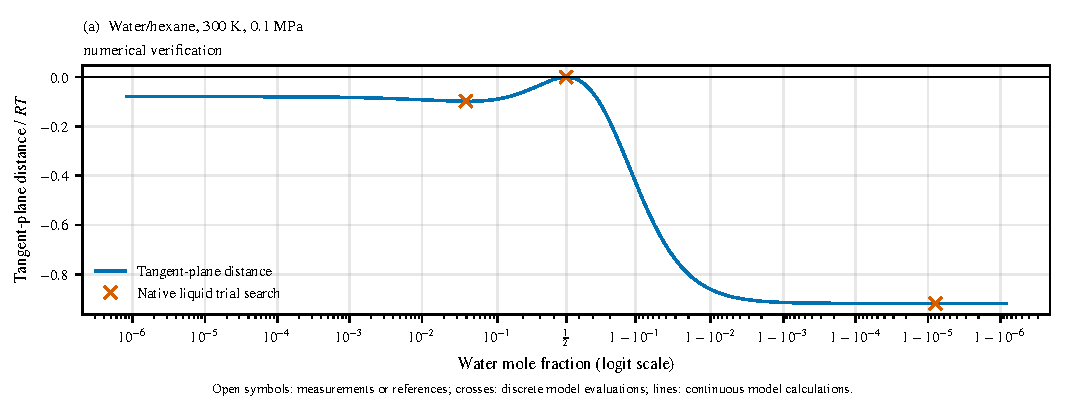
\includegraphics[width=0.96\linewidth]{F3-tpd-path}\par
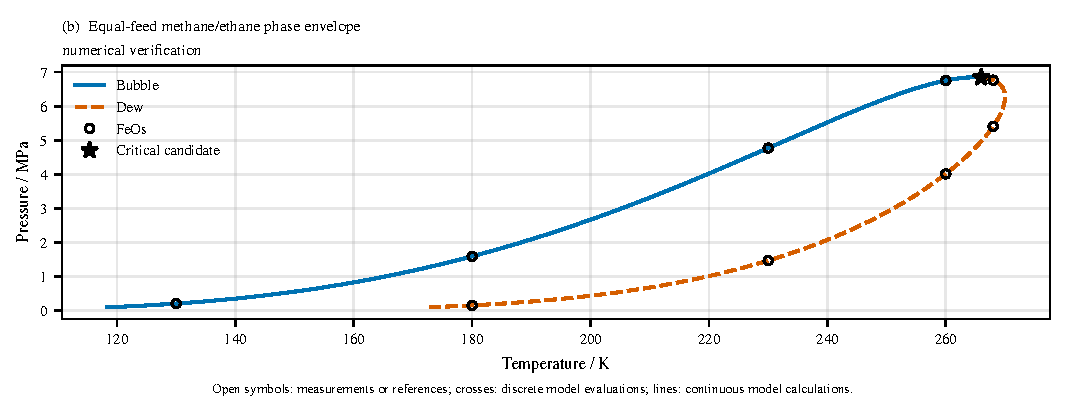
\includegraphics[page=1,width=0.96\linewidth]{F4-phase-envelope}
\caption{Phase search and envelope continuation (numerical verification).
Top: tangent-plane distance of a trial liquid against its water mole fraction for an equimolar water/hexane liquid at 300~K and 0.1~MPa, with crosses at the compositions returned by the liquid trial search of Algorithm~\ref{alg:discovery}.
The distance is zero at the feed and negative near both pure components, so the equimolar liquid is unstable as a single phase.
Bottom: bubble and dew curves of an equimolar methane/ethane mixture traced by continuation, with FeOs points and the critical-equation candidate; the remaining critical and bubble/dew comparisons are in the Supporting Information.}
\label{fig:search-envelope}
\end{figure}
